\begin{figure}[h!]
\centering
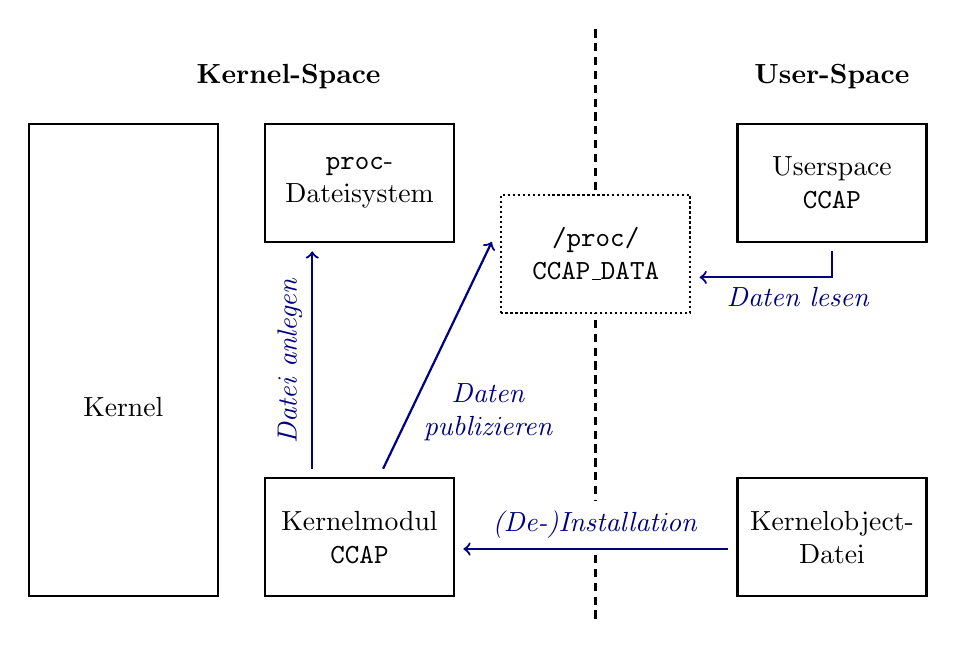
\begin{tikzpicture}[scale=0.6]
	
	% kernel space / user space
	\draw [very thick, densely dashed] (12,12) -- (12,-0.5);
	\node at (5.5,11) () {\textbf{Kernel-Space}};
	\node at (17,11) () {\textbf{User-Space}};
	
	% kernel core
	\draw [thick] (0,10) rectangle (4,0);
	\node at (2,4) () {Kernel};
	
	% module
	\draw [thick](5,2.5) rectangle (9,0);
	\node [align=center] at (7, 1.25) () {Kernelmodul\\ \texttt{CCAP}};
	
	% proc FS
	\draw [thick](5,10) rectangle (9,7.5);
	\node [align=center] at (7, 8.75) () {\texttt{proc}-\\Dateisystem};
		
	% kernel object file
	\draw [thick] (15,2.5) rectangle (19,0);
	\node [align=center] at (17,1.25) () {Kernelobject-\\Datei};
	
	% user space ccap
	\draw [thick] (15,10) rectangle (19,7.5);
	\node [align=center] at (17,8.75) () {Userspace\\ \texttt{CCAP}};
	
	% proc file
	\filldraw [white] (10,6) rectangle (14,8.5);
	\draw [thick, densely dotted] (10,6) rectangle (14,8.5);
	\node [align=center] at (12,7.25) () {\texttt{/proc/}\\ \texttt{CCAP\_DATA}};
	
	% installation
	\filldraw [white] (11,1) rectangle (13,2);
	\draw [thick, <-, black!50!blue] (9.2,1) -- (14.8,1) node [midway, above] {\textit{(De-)Installation}};
	
	% proc operations
	\draw [thick, ->, black!50!blue] (6,2.7) -- (6,7.3) node [rotate=90, midway, above] {\textit{Datei anlegen}};
	
	% read data
	\draw [thick, ->, black!50!blue] (17,7.3) -- (17,6.75) -- (14.2,6.75) node [near start, below] {\textit{Daten lesen}};
	
	\draw [thick, <-, black!50!blue] (9.8,7.5) -- (7.5,2.7) node [near end,xshift=1cm, align=center] {\textit{Daten}\\ \textit{publizieren}};
	
\end{tikzpicture}
\caption{Systemarchitektur des Programms \texttt{CCAP}}
\label{ccap}
\end{figure}
